\documentclass[twoside,a4paper]{refart}
\usepackage{t1enc} 
\usepackage[magyar]{babel}

\usepackage{graphicx}
\usepackage{listings}
\usepackage{hyperref}

\usepackage{caption}
\usepackage{subcaption}

\usepackage{lipsum}

\renewcommand{\lstlistingname}{Kódrészlet}
\renewcommand{\lstlistlistingname}{Kódrészletek listája}

\lstdefinestyle{mystyle}{
	numberstyle=\tiny,
	basicstyle=\ttfamily\footnotesize,
	breakatwhitespace=false,         
	breaklines=true,                                     
	keepspaces=true,                 
	numbers=left,                    
	numbersep=5pt,                  
	showspaces=false,                
	showstringspaces=false,
	showtabs=false,                  
	tabsize=2
}

\lstset{style=mystyle}


\title{Megoldandó feladat LogMeIn}
\author{Gesztesy Tamás}

\date{\today}
\emergencystretch1em  %

\pagestyle{myfootings}
\markboth{Megoldandó feladat \textrm{LogMeIn}}%
         {Megoldandó feladat \textrm{LogMeIn}}

\setcounter{tocdepth}{2}

\begin{document}

\maketitle

\begin{abstract}
	\begin{description}
		\item[A kapott feladat] On a network and dataset you are familiar with (the deeper is the better), visualize the loss surface, and give a list of potential candidate changes (that can affect the loss surface) and share your thoughts about them. Please, also send us the code you have used!
	\end{description}
\end{abstract}


A feladatot angol nyelven kaptam kézhez, ennek ellenére úgy döntöttem magyar nyelven fogom megoldani. Mivel a telefonos megbeszélés alapján úgy éreztem ez egy megengedhető könnyítés számomra. Nem vagyok jelentős tapasztalattal rendelkező Python programozó, de az állás kiírás alapján úgy éreztem, hogy a kódok átlátása és értelmezése az alapvető elvárás. Ezért úgy döntöttem egy létező kódot fogok felhasználni és feldolgozni. A témában megjelent egy releváns szakmai cikk Hao Li tollából.\cite{li2018visualizing} Ennek nyomán készült egy GitHub Repository\cite{VtLLoNN2020}, ami egyszerű és releváns leképezése volt a problémának. Ezt tervezem feldolgozni az alábbi munkában. A feladat megoldása során a PyCharm 2021.1.3 (Professional Edition) integrált fejlesztői környezettet, Anaconda Navigator 2.0.3 csomagkezelőt és a \LaTeX dokumentum szerkesztő nyelvet alkalmaztam.

\newpage

\tableofcontents

\newpage


%%%%%%%%%%%%%%%%%%%%%%%%%%%%%%%%%%%%%%%%%%%%%%%%%%%%%%%%%%%%%%%%%%%%

\section{Bevezetés}

\subsection{Az adathalmaz}
\label{adathalmaz}

A torchvision Python csomag biztosít több adathalmazt a neurális hálózatok betanításához. jelen esetben a CIFAR-10\cite{CIFAR10} adathalmaz lett felhasználva. Ez az adathalmaz tartalmaz 60 000 darab 32x32 pixel méretű színes képet. Amelyek tíz osztályba vannak sorolva, ezt szemlélteti, véletlen szerű mintákon keresztül, \aref{fig:cifar10} kép. A tanuló halmaz 50 000 képet tartalmaz, míg a teszt halmaz 10 000 képből áll. 
{\small \lstinputlisting[language=Python, firstline=5, lastline=6, caption={Adatok betőltése}, label=dataLoad]{code/dataloader.py}}

A betöltés alapvetően \aref{dataLoad}. kódrészletben történik a dataloader.py függvény környezetben. Itt egy egyszerű transzformációt is definiál az adatokon. Ez a [0,255] teret képezi le [0,1] térre.

A függvényt, aminek hívása ténylegesen elindítja a folyamatot láthatjuk \aref{dataloaderDef}. kódrészletben. Itt történik meg az objektum néhány tulajdonságának definiálása is. A tanuló halmaz minden epoch előtt meg lesz keverve, a teszt nem. A batch mérete 128 lesz, vagyis százhuszonnyolc minta kerül egy batch-be. Valamint látszik, hogy két szálon fog történni a betöltés.

{\small \lstinputlisting[language=Python, firstline=8, caption={Dataloader függvény}, label=dataloaderDef]{code/dataloader.py}}

\begin{figure}[th]
	\centering
	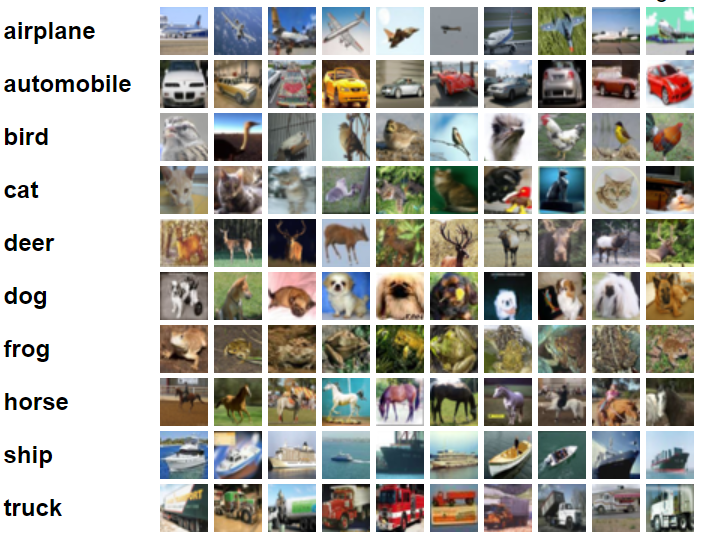
\includegraphics[width=0.6\linewidth]{image/CIFAR10}
	\caption[CIFAR-10]{CIFAR-10 adatbázis}
	\label{fig:cifar10}
\end{figure}


\subsection{A program futtatása}

A program futása két részből áll, előbb betanítjuk a neurális hálózatot, majd egy második programban megjelenítjük a Loss felületet.

\begin{description}
	
	\item[Main program]
	Alapvetően itt történik a hálózat tanítása. Az ehhez szükséges függvények külön fájlokba lettek rendezve. Ezeket természetesen először be kell hívni. Ez történik meg \aref{mainImnport}. kódrészletben. Először a neurális hálózatot importáljuk be, ebből persze csak egyet használ a program. Majd a véletlenszerű irányok létrehozásához szükséges függvény környezetet, végül pedig a Loss kiszámításához szükségeset.
	{\small \lstinputlisting[language=Python, lastline=5, caption={A szükséges blokkok importálása}, label=mainImnport]{code/main.py}}
	
	\Aref{mainDef}. kódrészletben látszik, hogy a ResNet56-al lett lefuttatva a program. Nagyjából három-négy óra futás idővel, egy darab Nvidia GeForce RTX 2080 videokártya használata mellett. Ezt követően három függvény hívás történik, amikkel a későbbi fejezetekben bővebben foglalkozom.
	
	{\small \lstinputlisting[language=Python, firstline=7, caption={A Main függvény}, label=mainDef]{code/main.py}}
	
	Most csak röviden.
	\begin{enumerate}
		\item A véletlenszerű irányok létrehozása
		\item A modell előkészítése
		\item Végül a Loss felület megjelenítéséhez szükséges adatok kiszámítása. 
	\end{enumerate}
	
	
	\item[Visualize program]
	Ez a program lényegében csak egy egyszerű megjelenítés, alapvető függvény blokkokat használ. A program egyetlen függvényt tartalmaz, aminek az eleje látható \aref{visualize}. kódrészletben.
	
	{\small \lstinputlisting[language=Python, firstline=11, lastline=39, caption={A Visualize függvény eleje}, label=visualize]{code/visualize.py}}
	
	Az adatok egy HDF5 fájlban (Hierarchical Data Format version 5) találhatóak és innen vannak megnyitva. Majd egy egyszerű megjelenítés történik. A függvény későbbi része hasonlóan elkészíti az adat megjelenítést, de ezek már elmentésre kerülnek pdf fájlokban.
	
\end{description} 

\section{Az alkalmazott neurális hálók}
	Itt nem fogok minden neurális hálózatra kitérni, aminek a használatát a program lehetővé teszi. Természetesen véges idő áll rendelkezésemre és a futási idők hosszúsága miatt nem tudtam többet lefuttatni. Mint \aref{mainImnport}. kódrészletben látszik két fájlban vannak szétszedve a hálózatok létrehozásához szükséges függvények. Az alexnet és a resnet fájlokban. Ez utóbbit fogjuk használni, de az alapvető működési elvek hasonlóak. Mivel \aref{mainDef}. kódrészletben látható módon a kód most egy ResNet56 hálót használ, így ezen keresztül lássuk most a futást. 

	{\small \lstinputlisting[language=Python, firstline=262, lastline=265, caption={resnet56}, label=resnet56nosshort]{code/resnet.py}}
	
	Tehát a meghívott függvényben beállításra kerül a mélység ami most 56.(lásd \aref{resnet56nosshort}. kódrészlet) Ezután meghívásra kerül a függvény, ami a hálózatot létre fogja hozni. Ennek első lépéseként egy alap blokkot ad át, ami a ResNet esetén mindig azonos lesz. Pontosabban kétféle verzióban létezik. Ebből az egyik tartalmaz egy rövidítést. Bár jelen esetben a rövidítést nem tartalmazó blokk kerül átadásra nézzük meg mégis a másik verziót. Ez ugyanis teljesen azonos a rövidítéstől eltekintve, ami könnyen azonosítható \aref{BasicBlock}. kódrészletben. Látszik, hogy négy alapréteg definiálása történik meg.
	
	{\small \lstinputlisting[language=Python, firstline=4, lastline=40, caption={BasicBlock}, label=BasicBlock]{code/resnet.py}}
	
	Tehát ezzel az alap blokkal kerül meghívásra a függvény, ami létre hozza majd a neurális hálózatot. Ebből az alábbi típusok léteznek.
	\begin{enumerate}
		\item ResNet
			\begin{enumerate}
				\item Bottleneck
				\item Bottleneck\_noshortcut
				\item ResNet
				\item ResNet\_cifar
				\item  WResNet\_cifar
			\end{enumerate}
		\item AlexNet
	\end{enumerate}
	
	Tekintsük át röviden a használt ResNet hálózatot, ami kifejezetten a CIFAR adathalmazhoz készült. A bemenetek képek, ehhez egy 2D konvolúciós réteget és egy 2D Batch normálási réteget hoz létre. Ezt követik a belső rétegek. Majd létrehoz egy lineáris réteget, ami a kimenetek, osztályok számának megfelelően kerül definiálásra. Lásd \aref{ResNetcifar}. kódrészletet.
	
	{\small \lstinputlisting[language=Python, firstline=139, lastline=167, caption={ResNet\_cifar}, label=ResNetcifar]{code/resnet.py}}
	
	Ezzel el is készült a neurális hálózat, amit felhasználunk a tanítás során.
	
\section{Véletlenszerű irányok definiálása}

	A következő lépés a véletlenszerű irányok definiálása. Ehhez meghívjuk a create\_random\_directions függvényt, aminek átadjuk a létrehozott hálózatot.(lásd \ref{mainDef}. kódrészletet) Mint \aref{directions}. kódrészletben látszik maga a függvény elég egyszerű.
	
	{\small \lstinputlisting[language=Python, firstline=4, lastline=8, caption={create\_random\_directions}, label=directions]{code/directions.py}}
	
	A meghívott függvény, ami ténylegesen létrehozza az irányokat \aref{direction}. kódrészletben látható. Három részre lehet bontani a működést.
	\begin{enumerate}
		\item A sulyok létrehozása
		\item Az irány létrehozása
		\item Az irány normálása
	\end{enumerate}
	
	{\small \lstinputlisting[language=Python, firstline=11, lastline=16, caption={create\_random\_direction}, label=direction]{code/directions.py}}
	
	A súlyokat értelemszerűen a már korábban definiált modellből nyerjük vissza. Lásd \aref{getweights}. kódrészletet.
	
	{\small \lstinputlisting[language=Python, firstline=19, lastline=20, caption={get\_weights}, label=getweights]{code/directions.py}}
	
	Ezek közül véletlenszerűen választunk \aref{getrandomweights}. kódrészletben.
	
	{\small \lstinputlisting[language=Python, firstline=23, lastline=24, caption={get\_random\_weights}, label=getrandomweights]{code/directions.py}}
	
	Majd végrehajtjuk a normalizálást \aref{normalizedirectionsforweights}. kódrészletben.
	
	{\small \lstinputlisting[language=Python, firstline=27, lastline=36, caption={normalize\_directions\_for\_weights}, label=normalizedirectionsforweights]{code/directions.py}}
	
	Ekkor merül fel a probléma, hogy a használt kód nem köti ki az ortogonalitást, mint elvárt feltételt. Erre ad megoldást \aref{FilterOrthogonalization}. kódrészlet. Ez egy a témával foglalkozó cikkből\cite{jae2019VLLoDNN} származik. Ebben a kódban egy egyszerű gauss eloszlást használt a szerző és QR felbontással ortogonalizálta az irányokat.
	
	{\small \lstinputlisting[language=Python, caption={Filter\_Orthogonalization}, label=FilterOrthogonalization]{code/Filter_Orthogonalization.py}}
	
	Ez lehet egy ideális kiegészítése a fenti kódnak. Ez egy könnyen kivitelezhető hozzátétel. Viszont a futásidő hosszúsága, miatt ennek tesztelésére nekem most nem volt lehetőségem.
	
\section{A modell előkészítése}  

	Először nézzük tehát meg a függvényt, ami az előkészítést végzi \aref{preparetrainedmodel}. kódrészletben. Az első, ami szembetűnik, hogy a függvény környezet használ egy globális változót ami negyvenben határozza meg az epoch-ok számát. Maga a függvény csak azt kezeli, hogy létezik-e már a modell. Ebben az esetben ugyanis nincsen szükség arra, hogy újra fusson.
	
	{\small \lstinputlisting[language=Python, firstline=7, lastline=17, caption={prepare\_trained\_model}, label=preparetrainedmodel]{code/train_model.py}}
	
	Ez követően nézzük meg magát a tanító függvényt, ami \aref{TrainFuggvenyElo}. kódrészletben látható. Ez első lépésként meghívja \aref{adathalmaz}. fejezetben már részletezett adatbetöltő függvényt. Ezt követően megvizsgálja, hogy rendelkezésre áll egy videokártya vagy CPU-val kell megoldani a tanítást. Definiálásra kerül Cross Entropy Loss kritérium\cite{CrossEntropyLoss}. Valamint az optimalizálás Stochastic Gradient Descent módszerrel\cite{sutskever2013importance}. Végül pedig néhány üres vektor, amik később még szükségesek lesznek. 
	
	{\small \lstinputlisting[language=Python, firstline=19, lastline=33, caption={Train függvény előkészitése}, label=TrainFuggvenyElo]{code/train_model.py}}
	
	\Aref{TrainFuggTorzs}. kódrészletben van egy for ciklusom, ami annyiszor fog futni, ahány az epoch-ok száma. 
	\begin{enumerate}
		\item Első lépésként történik egy tanítás.
		\item Egy for ciklusban kiszámoljuk a loss-t és az accuracie-t minden képre.
		\item Számolunk egy átlagos loss-t és accuracie-t.
		\item Átváltunk a validációs halmazra.
		\item Ura számoljuk a loss-t és az accuracie-t.
		\item Kiírjuk a kapott értéket.
		\item Elmentjük az értéket.
	\end{enumerate}
	
	{\small \lstinputlisting[language=Python, firstline=34, caption={Train függvény tőrzs rész}, label=TrainFuggTorzs]{code/train_model.py}}
	
	Ezt követően a függvény már csak ábrázolja a kapott értékeket és elmenti őket.
	
\section{A Loss felület kiszámítása}
	
	A loss felület kiszámításáért felelős függvény környezet tartalmazza magát calulate\_loss\_landscape függvényt, ez látszik \aref{calulatelosslandscape}. kódrészletben.
	
	{\small \lstinputlisting[language=Python, firstline=8, lastline=40, caption={calulate\_loss\_landscape}, label=calulatelosslandscape]{code/calc_loss.py}}
	
	Ennek első lépése egy függvény hívás, ez a függvény látható \aref{setupsurfacefile}. kódrészletben. Ebben fogjuk meghatározni a kiinduló paramétereket. Jelen esetben egy -1 és 1 közötti felületet. Majd létrehozunk az adatok tárolására egy fájlt, ami tartalmazni fogja az induló értékeket. Vagyis minden x és y koordináta párhoz hozzárendel egy egyes Loss-t és egy egyes accuracie-t.
	
	{\small \lstinputlisting[language=Python, firstline=42, lastline=69, caption={setup\_surface\_file}, label=setupsurfacefile]{code/calc_loss.py}}
	
	Ezt követően az calulate\_loss\_landscape lekérik a modell súlyokat. Majd megnyitja az előbb létrehozott fájlt. Majd indexet rendel az egyes koordinátákhoz és egy for ciklussal végig megy rajtuk. Ennek első lépéseként a koordináták alapján újra számolja a modell paramétereket. Lásd \aref{overwriteweights}. kódrészletben. 
	
	{\small \lstinputlisting[language=Python, firstline=83, caption={overwrite\_weights}, label=overwriteweights]{code/calc_loss.py}}
	
	Ezt követően Kiszámolja a loss-t és az accuracie-t. Ez a tanító függvényben látotthoz hasonlóan történik. Egy test\_model.py függvénykörnyezetben. Ez természetesen már csak a teszt adatokat tölti be a tanuló halmazt nem. Majd az adatok elmentésre kerülnek.
	
\section{Konklúzió}
	A fentebb már említett cikk\cite{jae2019VLLoDNN} szerzője foglalkozik a témával, hogy a különböző felbontások és ortogonalizálások jelentős kihatással lehetnek a Loss felületre. Ez pedig kérdéseket vett fel, az ebből levont következtetésekkel kapcsolatban. Az alább látható egyszerű véletlen irányokkal készült felületek, ennek ellenére adhatnak kiindulási alapot a megfelelő paraméterezés megtalálásához. Először egy AlexNet (lásd \ref{fig:alexnettrainloss3dsurface} ábra) háló volt betanítva az adathalmazra. Ez egy viszonylag egyszerű felületet mutat, aminek minimum helye a nulla pontban látszik. A második felület pedig egy ResNet18 hálót ábrázol, ami jelentősen komplexebb felületet mutat. Lásd \ref{fig:resnet18noshortcuttestloss3dsurface} ábra. Nem is lehet egyértelműen meghatározni egy minimum pontot. 
	\begin{figure}[th]
		\centering
		\caption{AlexNet és ResNet18}
		\label{fig:AlexNetResNet18}
		\begin{subfigure}[t]{0.49\linewidth}
			\centering
			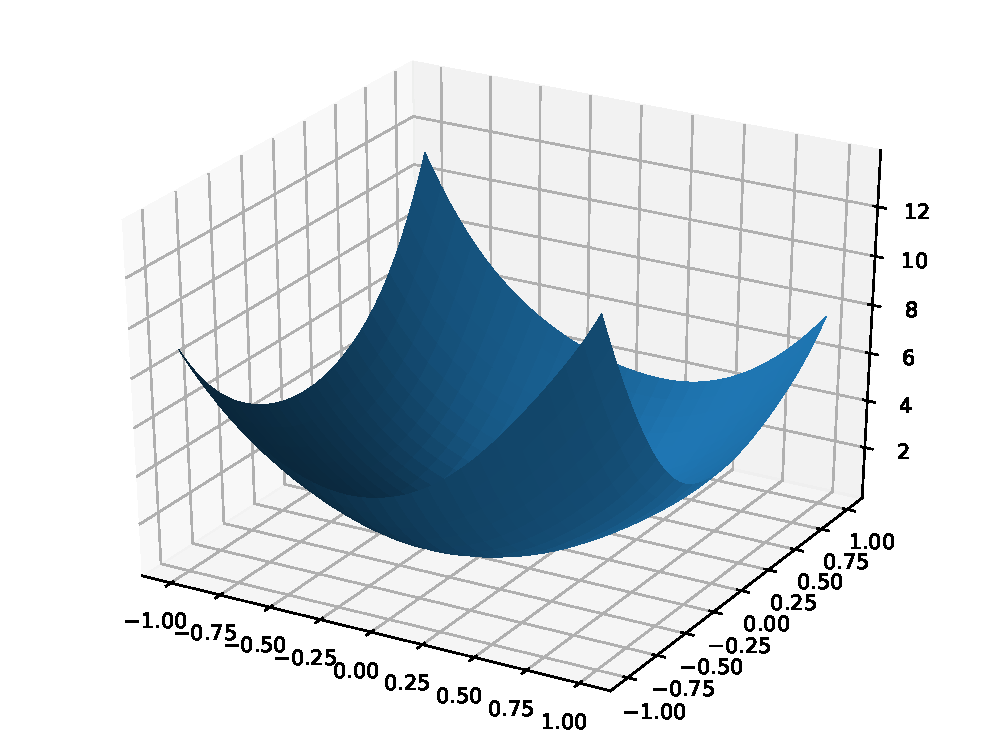
\includegraphics[width=0.9\linewidth]{image/alexnet_train_loss_3dsurface}
			\caption[AlexNet]{AlexNet Train Loss 3D Surface}
			\label{fig:alexnettrainloss3dsurface}
		\end{subfigure}
		\hfil
		\begin{subfigure}[t]{0.49\linewidth}
			\centering
			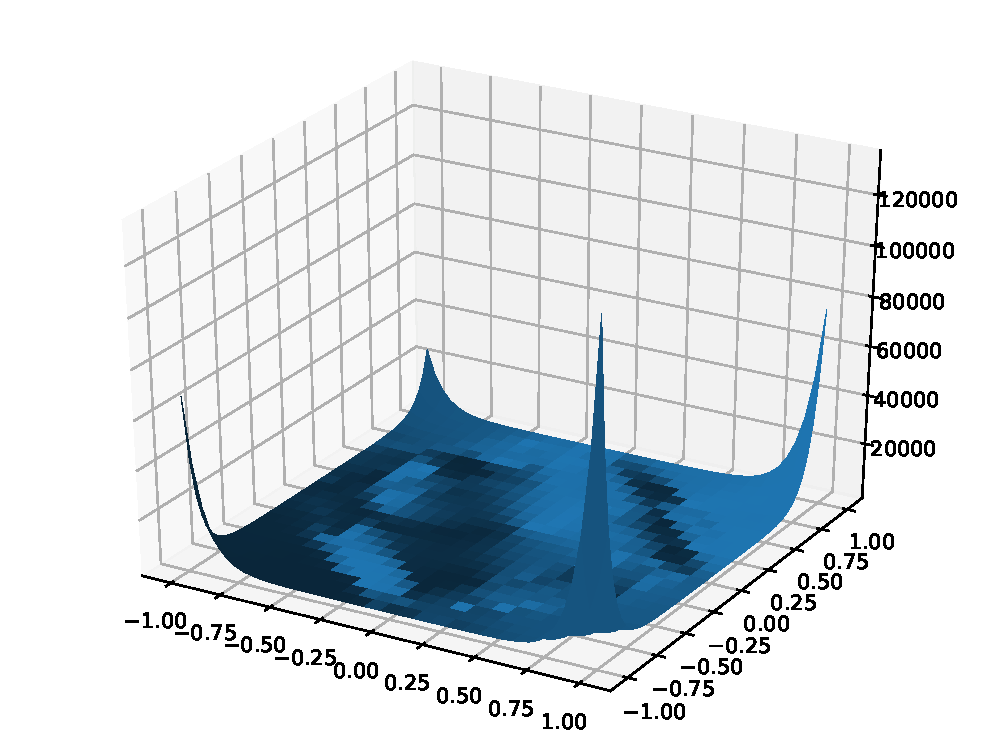
\includegraphics[width=0.9\linewidth]{image/resnet18_no_shortcut_test_loss_3dsurface}
			\caption[ResNet18]{ResNet18 no shortcut test Loss 3D Surface}
			\label{fig:resnet18noshortcuttestloss3dsurface}
		\end{subfigure}
	
	\end{figure}

	\Aref{fig:resnet56}. ábra pár ugyanazt a ResNet56 hálózat típust mutatja, azonos paraméterezés mellett. Mégis látszik, hogy a kerülő utak használata eltérő felületet eredményez. Ez egyébként általánosságban is látszik a négy ábrán, hogy a kerülő utak használata minden esetben jelentősen komplexebb felületet eredményez.

	\begin{figure}[th]
		\centering
		\caption{ResNet56}
		\label{fig:resnet56}
		\begin{subfigure}[t]{0.49\linewidth}
			\centering
			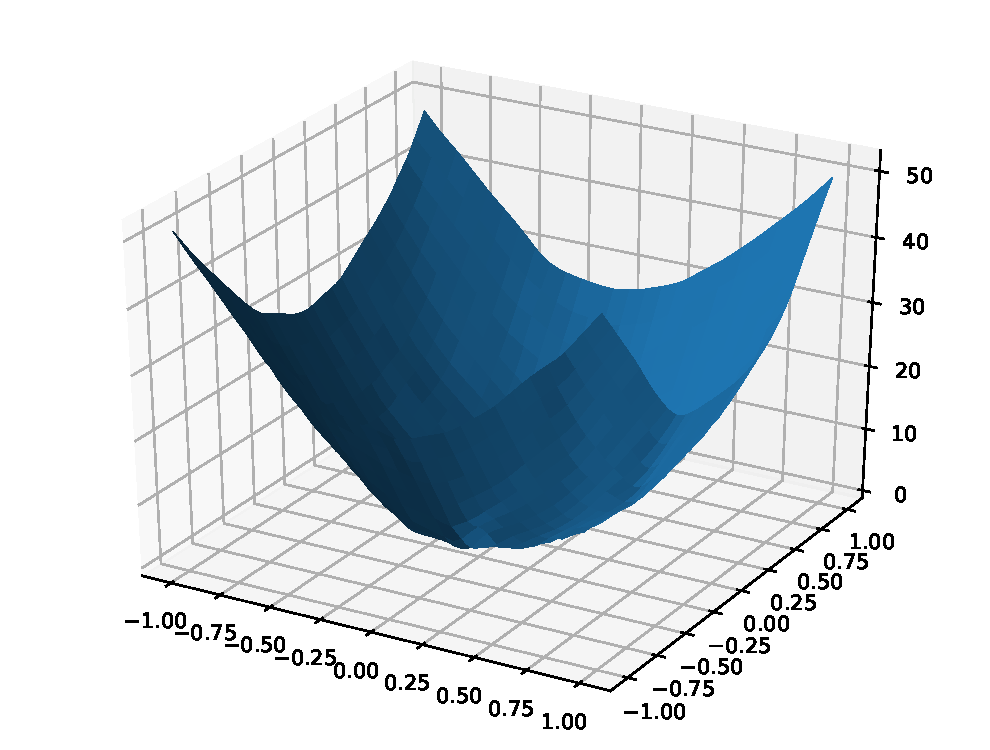
\includegraphics[width=0.9\linewidth]{image/resnet56_test_loss_3dsurface}
			\caption[ResNet56]{ResNet56 test loss 3D Surface}
			\label{fig:resnet56testloss3dsurface}
		\end{subfigure}
		\hfil
		\begin{subfigure}[t]{0.49\linewidth}
			\centering
			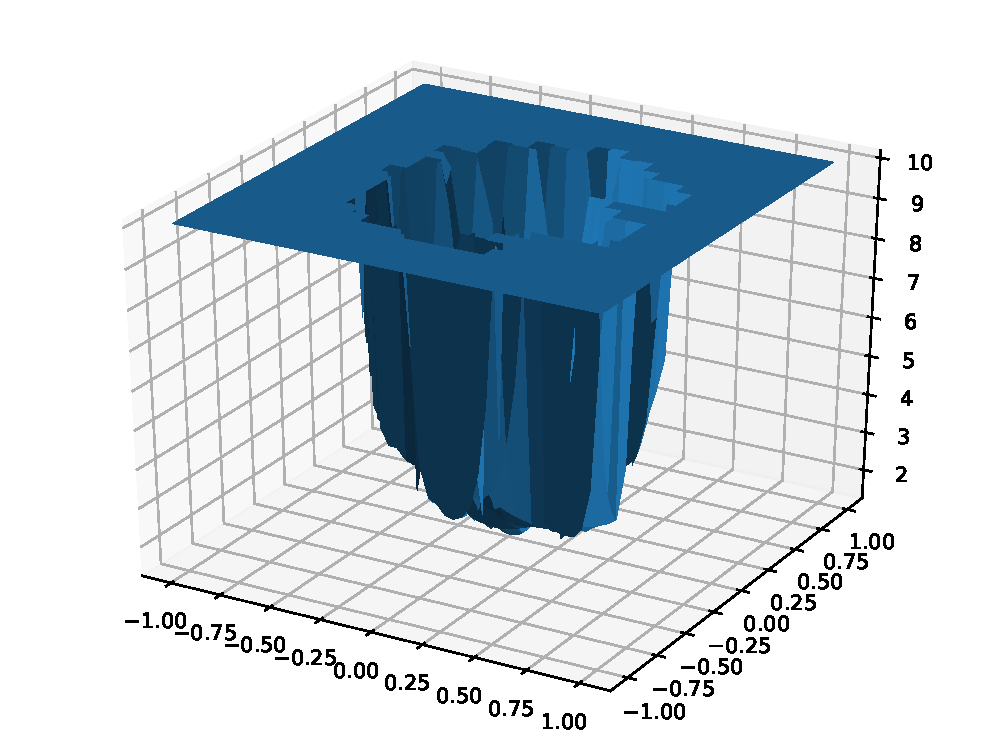
\includegraphics[width=0.9\linewidth]{image/resnet56_no_short_test_loss_3dsurface}
			\caption[ResNet56 no shortcut]{ResNet56 no shortcuts test loss 3D Surface}
		\end{subfigure}
		
	\end{figure}
	
\newpage

\addcontentsline{toc}{section}{\lstlistlistingname}
\lstlistoflistings

\addcontentsline{toc}{section}{Hivatkozások}
\bibliographystyle{unsrt}
\bibliography{hivatkozas}

\end{document}
